\documentclass[12pt,aspectratio=169]{beamer}

\usetheme[progressbar=frametitle]{metropolis}
\usepackage{appendixnumberbeamer}

\usepackage{booktabs}
\usepackage[scale=2]{ccicons}

\usepackage{pgfplots}
\usepgfplotslibrary{dateplot}

\usepackage{xspace}
\newcommand{\themename}{\textbf{\textsc{metropolis}}\xspace}

\usepackage{datetime}

\usepackage{threeparttable}
\usepackage{multirow}
\usepackage{tabularx}
\usepackage[]{siunitx}
\usepackage{makecell}
\usepackage{diagbox}
\usepackage[absolute,overlay]{textpos}

% Grid
%\usepackage[texcoord,grid,gridunit=mm,gridcolor=red!10,subgridcolor=green!10]{eso-pic}


\usepackage{pifont}
\newcommand{\cmark}{\ding{51}}%
\newcommand{\xmark}{\ding{55}}%
\newcommand{\eqmark}{{\bf \(\approx\)}}

\definecolor{lightgray}{rgb}{0.83, 0.83, 0.83}
\definecolor{lightblue}{rgb}{0.68, 0.85, 0.9}
\definecolor{lightgreen}{rgb}{0.56, 0.93, 0.56}
\definecolor{thistle}{rgb}{0.85, 0.75, 0.85}


\usepackage{minted}
\setminted{fontsize=\scriptsize}

\newdate{dateSoutenance}{04}{11}{2022}


\usepackage[backend=biber,
            defernumbers=true,
            sorting=ynt,
            %style=numeric,
            style=authortitle,
            %style=draft,
            backref=true]{biblatex}
\addbibresource{../bibliography.bib}


\title{Generic programming in modern C++ for\\ Image Processing}
%\subtitle{}
\date{Thesis Defense --- \displaydate{dateSoutenance}}
\author{\textbf{Michaël Roynard} \hspace{1cm} Supervision: \emph{Edwin Carlinet} \hspace{1cm} Direction: \emph{Thierry
Géraud}}
\institute{EPITA Research Laboratory (LRE) --- Le Kremlin Bicêtre, France}
\titlegraphic{

\includegraphics[width=.2\textwidth]{../images/logo-edite.pdf}\hfill

\includegraphics[width=.2\textwidth]{../images/epita.pdf}\hfill

\includegraphics[width=.2\textwidth]{../images/lre-logo.png}\hfill

\includegraphics[width=.2\textwidth]{../images/Logo_of_Sorbonne_University.pdf}
}

\makeatletter
\setbeamertemplate{title page}{
  \begin{minipage}[b][\paperheight]{\textwidth}
    \vfill%
    \ifx\inserttitle\@empty\else\usebeamertemplate*{title}\fi
    \ifx\insertsubtitle\@empty\else\usebeamertemplate*{subtitle}\fi
    \usebeamertemplate*{title separator}
    \ifx\beamer@shortauthor\@empty\else\usebeamertemplate*{author}\fi
    \ifx\insertdate\@empty\else\usebeamertemplate*{date}\fi
    \ifx\insertinstitute\@empty\else\usebeamertemplate*{institute}\fi
    \vfill
    \ifx\inserttitlegraphic\@empty\else\inserttitlegraphic\fi
    \vspace*{1cm}
  \end{minipage}
}
\makeatother

\begin{document}

\maketitle

\begin{frame}{Overview}
  \setbeamertemplate{section in toc}[sections numbered]
  \tableofcontents[hideallsubsections]
\end{frame}

%
%
%

\section[General Introduction]{General Introduction}

\begin{frame}[fragile]{Image processing nowadays}
  \begin{itemize}
    \item Image processing is everywhere, in most of the devices (computer, phone, embedded, etc.)
    \item Applications are multiples (medical imaging, social network filters, facial recognition, etc.).
    \item Every industry and research domain is using it (production line automation, automatic document reading, social network apps, etc.)
    \item Image Processing is costly in resources. Performances are crucial.
  \end{itemize}
  \begin{figure}[bl]
    \hfill
    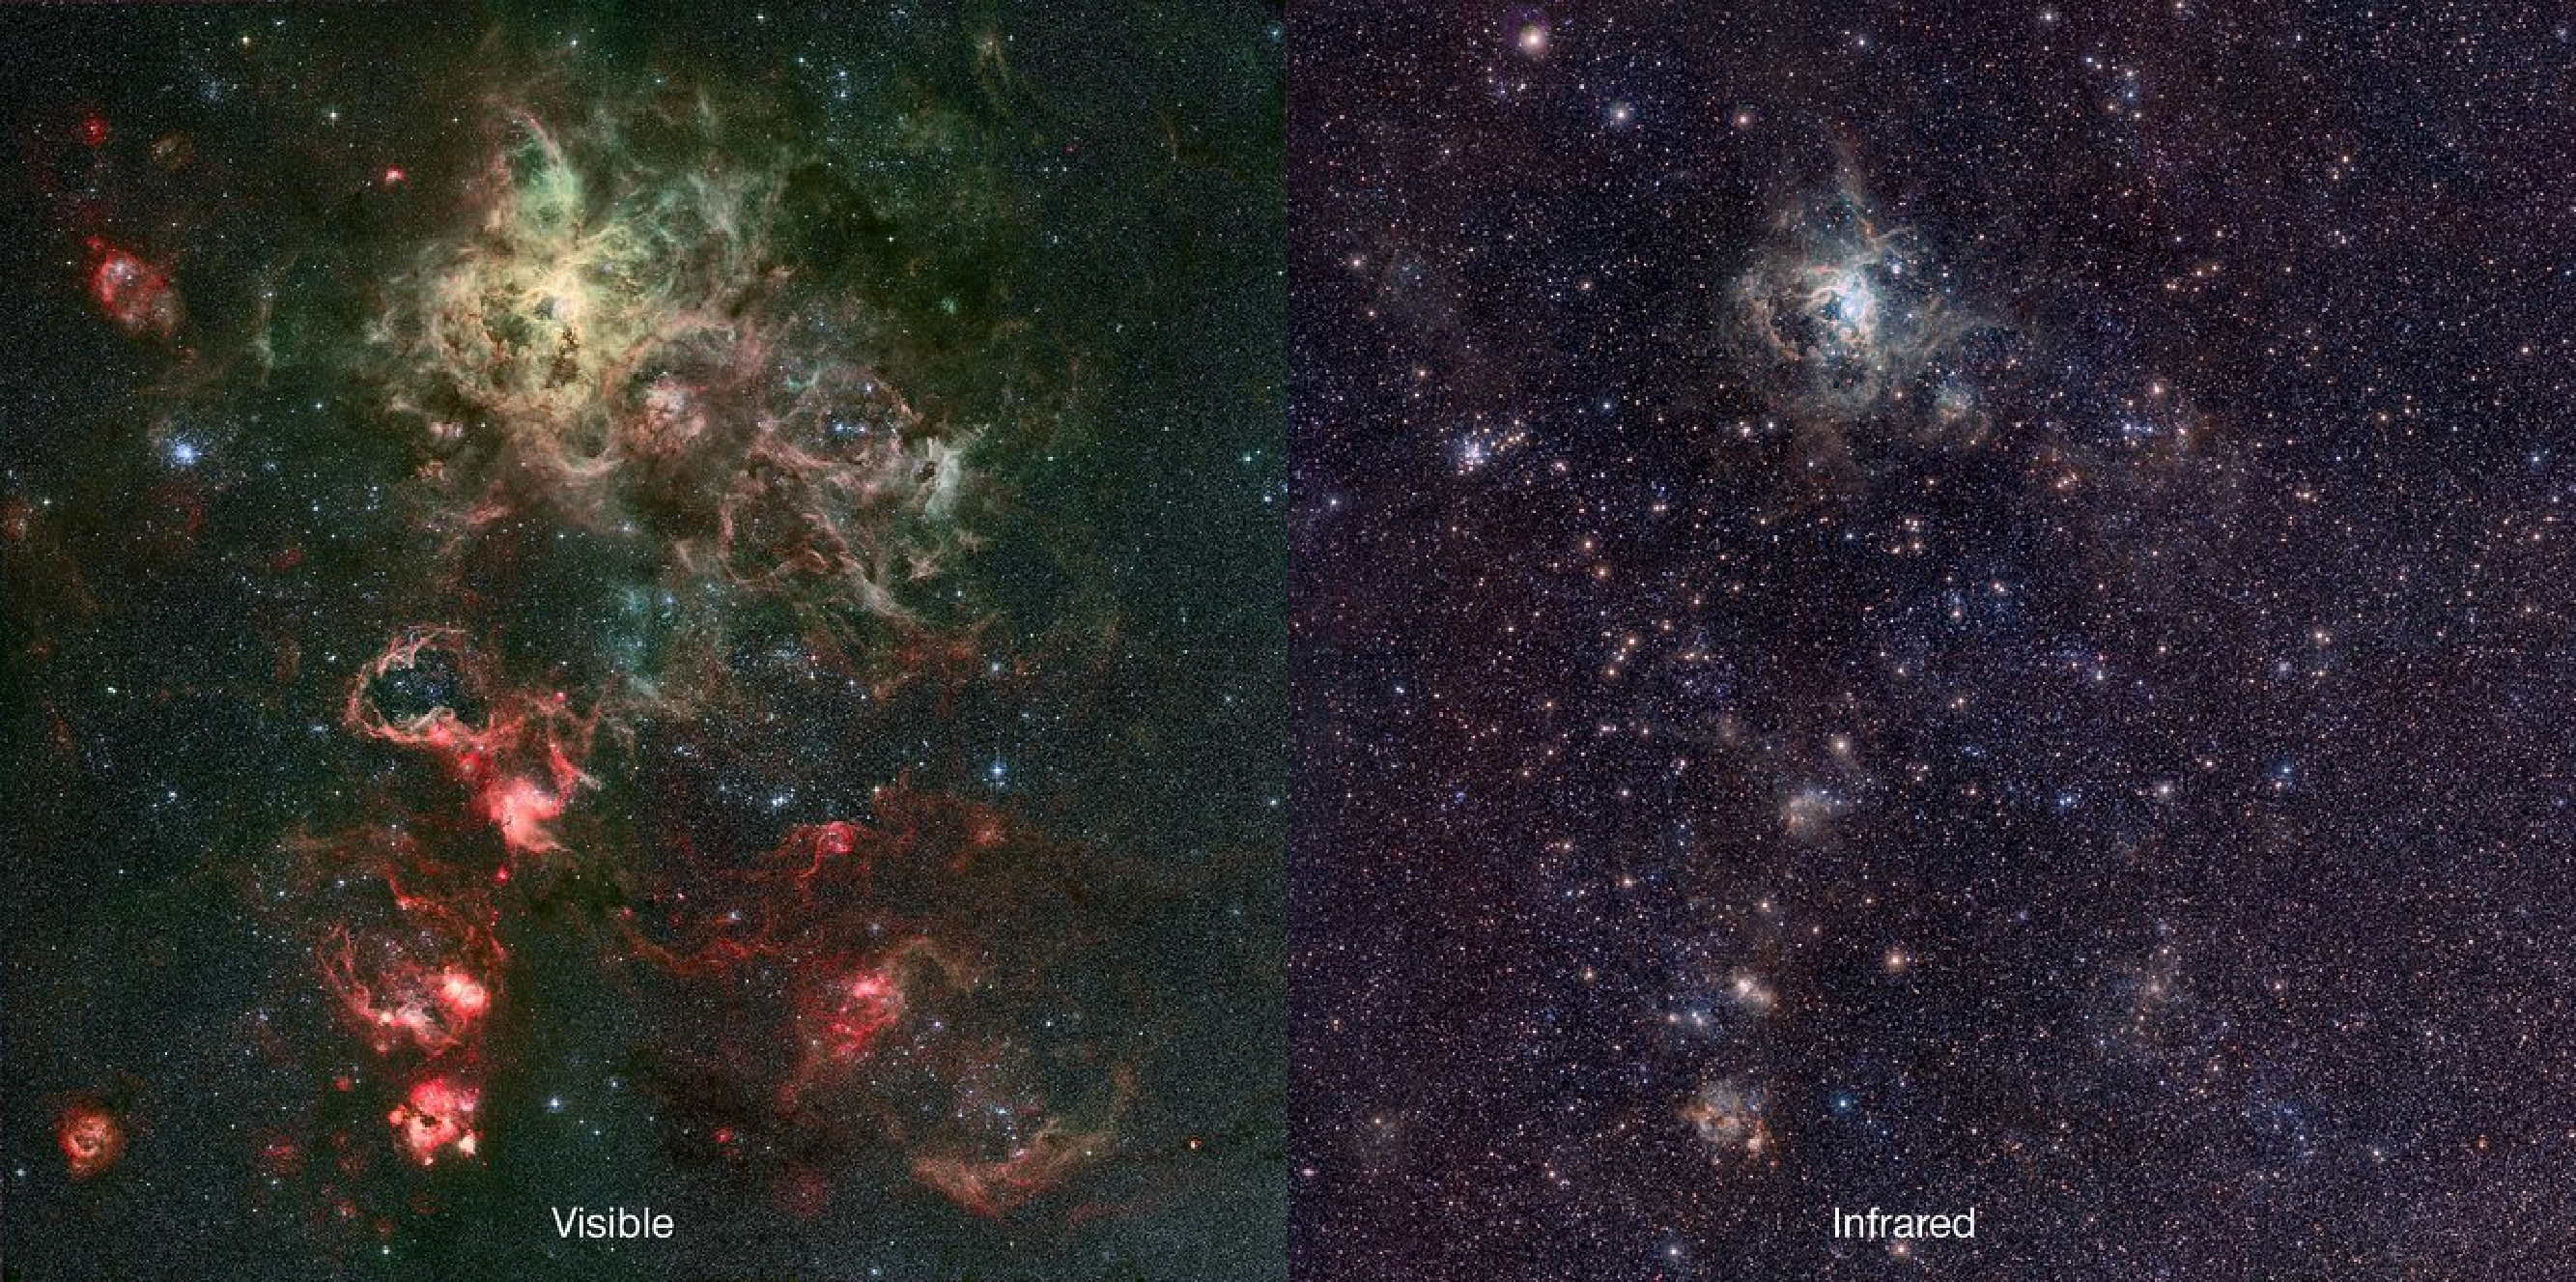
\includegraphics[height=3cm]{../illustrations/rgb_infrared.pdf}
    \hfill
    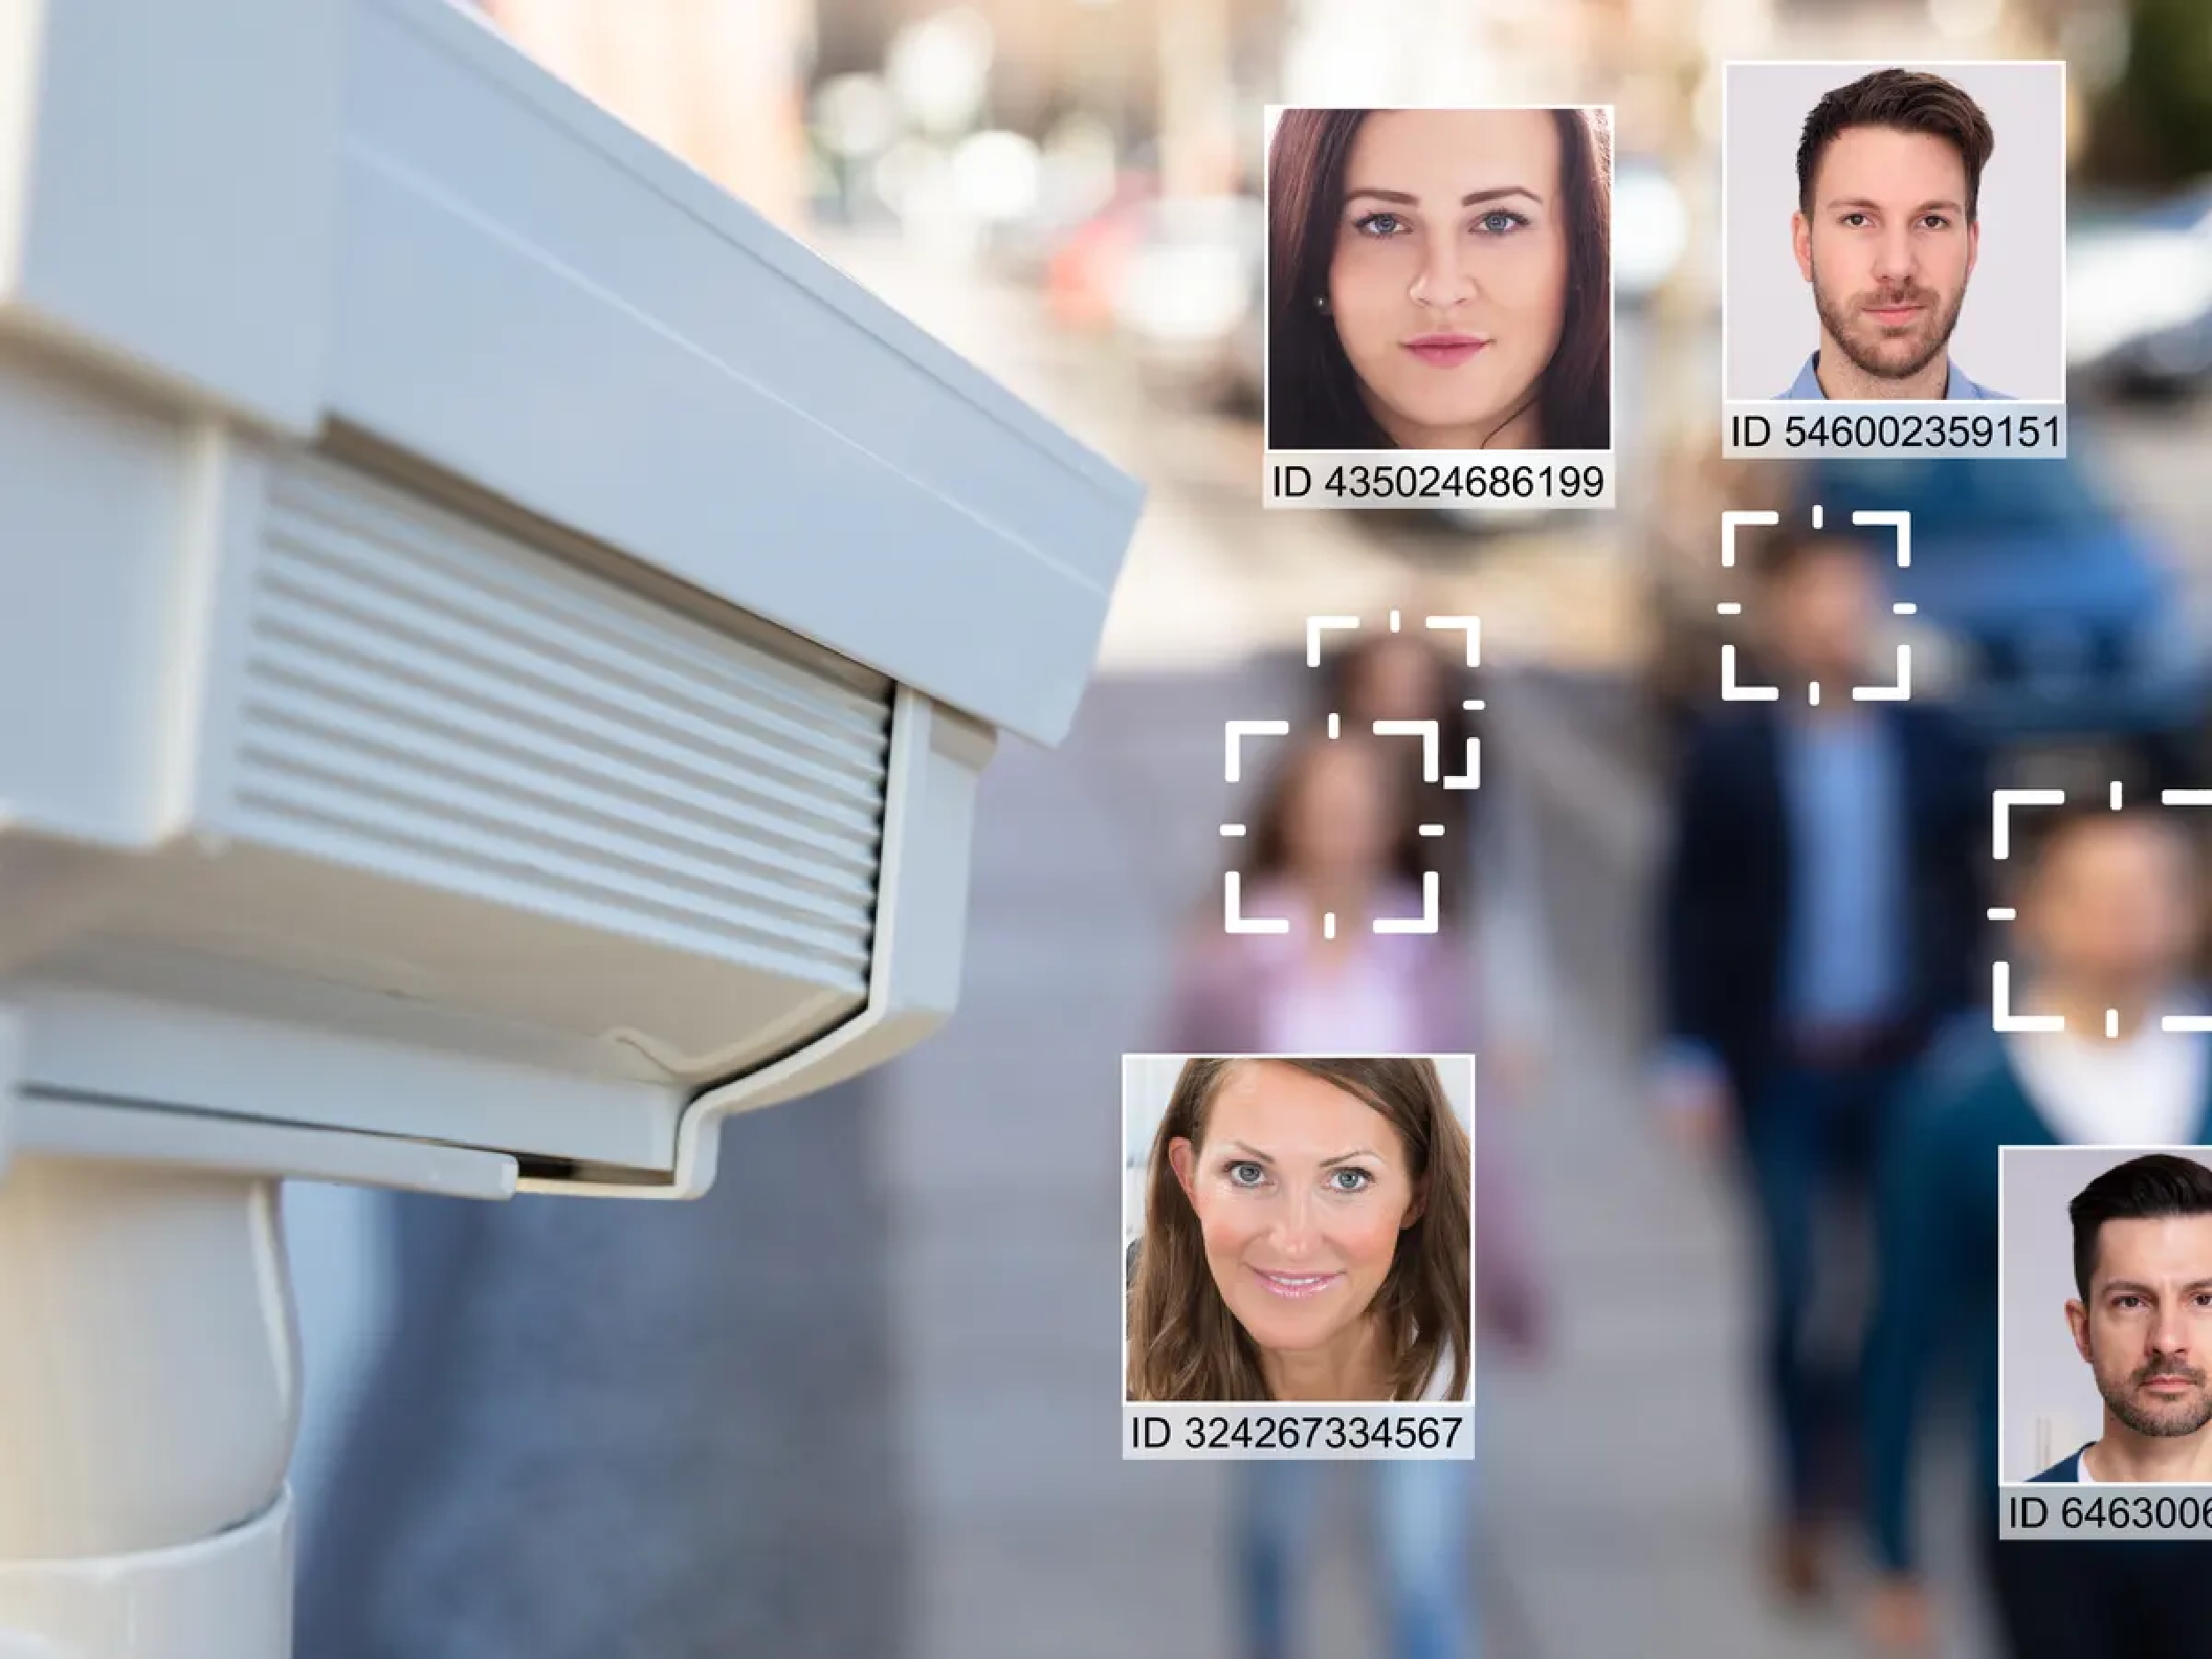
\includegraphics[height=3cm]{../illustrations/camera.pdf}
    \hspace{1cm}
  \end{figure}
\end{frame}

\begin{frame}[fragile]{Image processing nowadays}
  \begin{alertblock}{Different data types and algorithms}
    \begin{itemize}
      \item image-ND, hexagonal grid, cubical complexes value, etc.
      \item pixel-wise algorithms, local algorithms (convolution), global algorithms (propagation)
    \end{itemize}
  \end{alertblock}
  \begin{figure}[bl]
    \hfill
    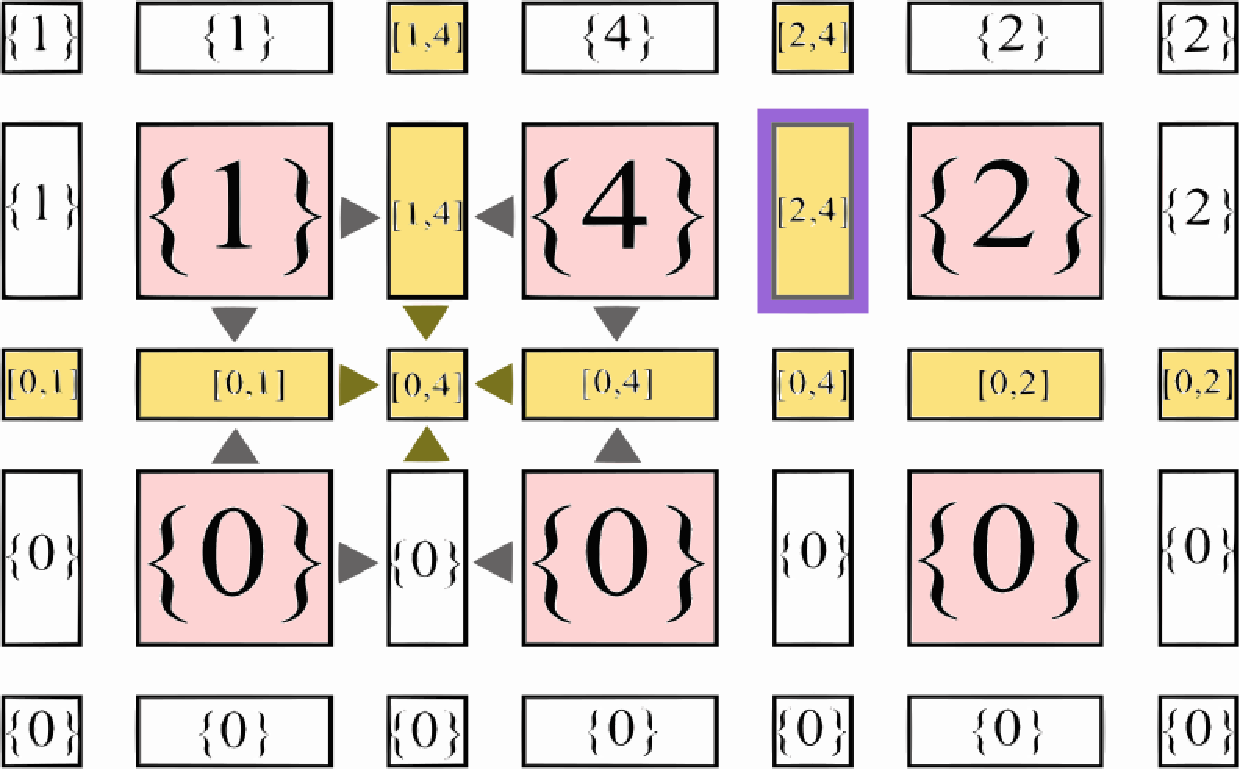
\includegraphics[height=3cm]{../illustrations/cubical_complex.pdf}
    \hfill
    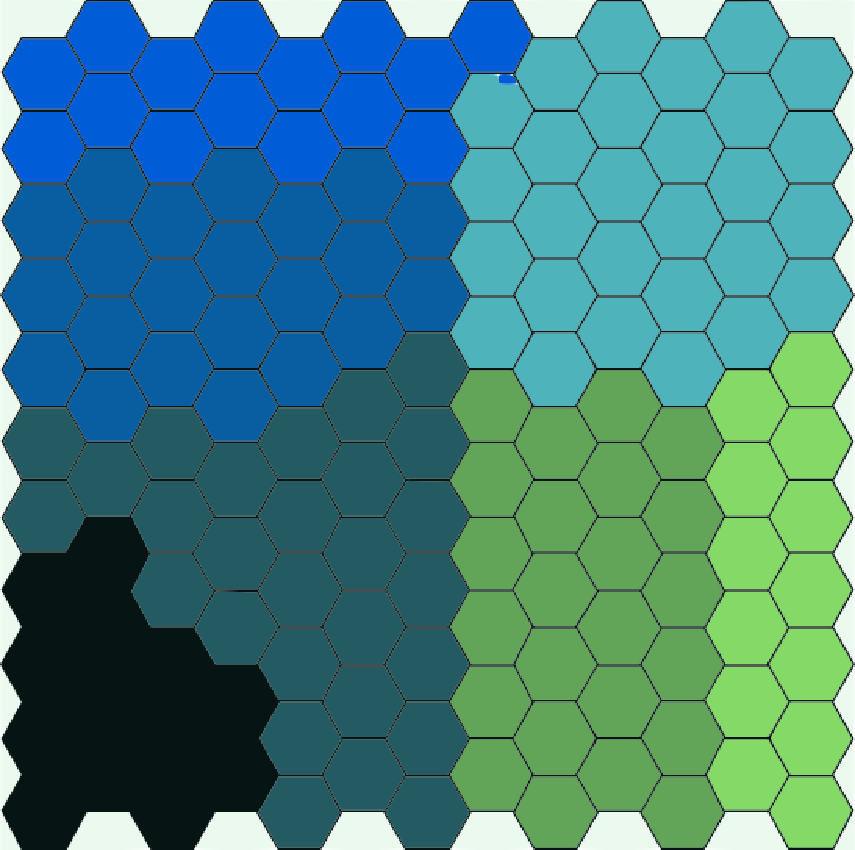
\includegraphics[height=3cm]{../illustrations/hexagonal_grid2.pdf}
    \hspace{1cm}
  \end{figure}
\end{frame}

\begin{frame}[fragile]{Image processing nowadays}
  \begin{alertblock}{Different user profiles and their use cases}
    \begin{itemize}
      \item The end user (non-programmer, wants UI interface).
      \item The practitioner (end user of an image processing library).
      \item The contributor (advanced user of a library familiar with its internals).
      \item The maintainer (founder/creator of the library or took it over to make it grow).
    \end{itemize}
  \end{alertblock}

  Our work is aimed toward the \emph{practitioner}, the \emph{contributor} and the \emph{maintainer}.
\end{frame}

\begin{frame}[fragile]{Image processing nowadays}
  \begin{alertblock}{Different tools}
    \begin{itemize}
      \item Graphic editors (GIMP, Photoshop).
      \item Command line utilities (ImageMagick, GraphicsMagick or MegaWave).
      \item Visual programming environment (Mathcad).
      \item Integrated environment (Matlab, Scilab, Octave, Mathematica and Jupyter).
      \item Package for Python (SciPy, NumPy, Scikit-image, Pillow or OpenCV bindings, via PyPi or Conda).
      \item Programming libraries (IPP, ITK, Boost.GIL, Vigra, Higra, GrAL, DGTal, OpenCV, CImg, Video++, Generic Graphic
            Library, Milena and Olena.
            %\item Domain Specific Languages (DSL)~\footcite{deursen.2000.DSL} (Eigen, Blaze, Blitz++ or Armadillo via C++
            %      Expression template~\footcite{veldhuizen.1995.expression}, or Halide and SYCL with their own toolchain).
      \item Domain Specific Languages (DSL) (Eigen, Blaze, Blitz++ or Armadillo via C++ Expression template, or Halide
            and SYCL with their own toolchain).
    \end{itemize}
  \end{alertblock}
\end{frame}

\begin{frame}[fragile]{Need of Genericity for image processing}
  \begin{figure}[htbp]
    \raggedright\small
    \begin{tabular}{cccc}
                                                                              & image 2D
                                                                              & graph    & mesh \\[5pt]
      input:                                                                  &
      \fbox{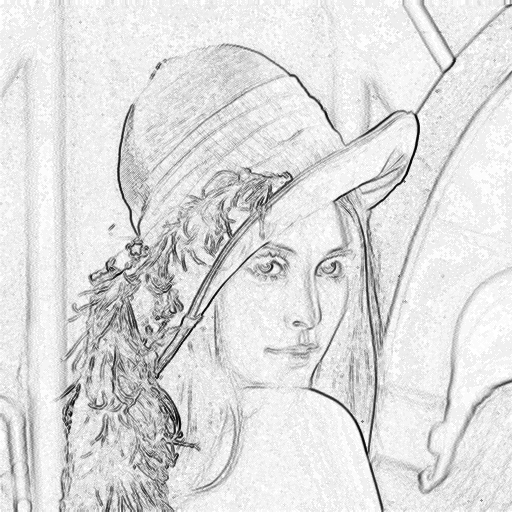
\includegraphics[width=.14\linewidth]{../figures/geninput-000b}}  &
      \fbox{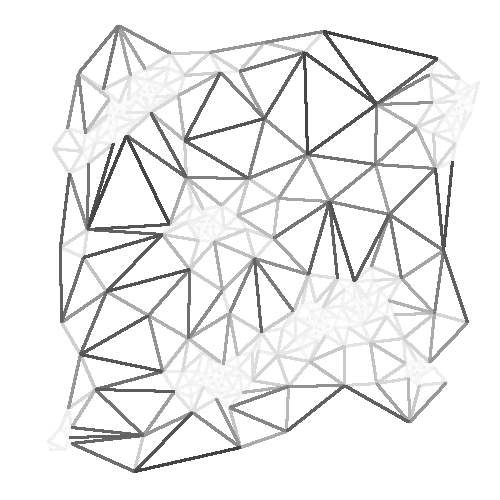
\includegraphics[width=.14\linewidth]{../figures/geninput-001b}}  &
      \fbox{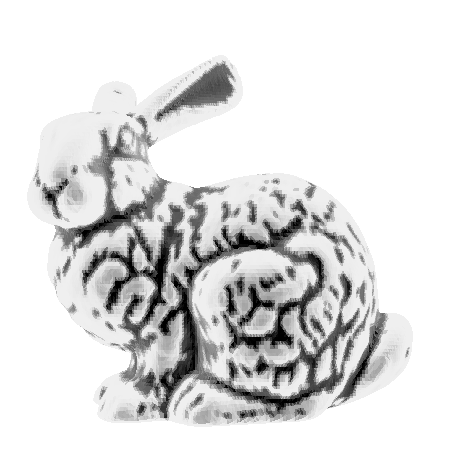
\includegraphics[width=.14\linewidth]{../figures/geninput-002b}}
      \\[5pt]
      %
      output:                                                                 &
      \fbox{
\includegraphics[width=.14\linewidth]{../figures/genoutput-000}}  &
      \fbox{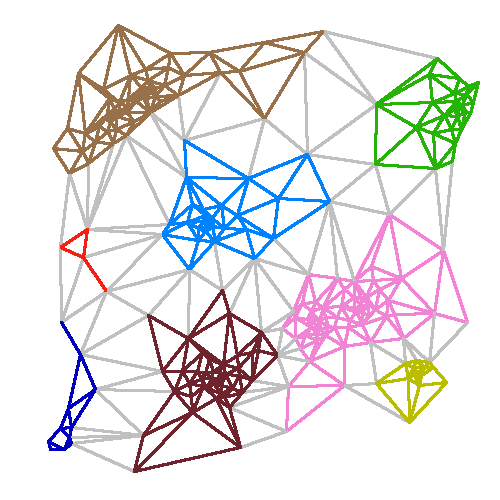
\includegraphics[width=.14\linewidth]{../figures/genoutput-001b}} &
      \fbox{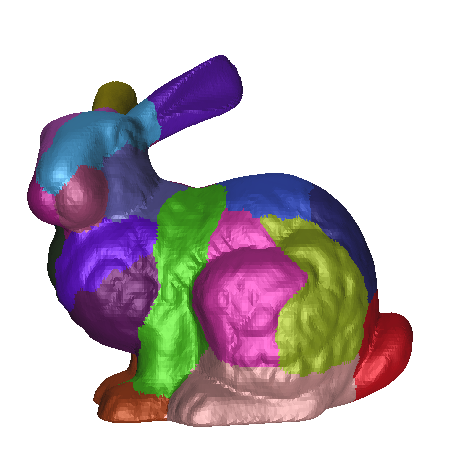
\includegraphics[width=.14\linewidth]{../figures/genoutput-002b}}
      \\
    \end{tabular}
    \label{fig:type.vs.algo}
    \caption{Watershed algorithm applied to three different image types.~\footcite{levillain.2014.ciarp}}
    %\vspace{-0.5cm}
    %\text{\textbf{Algorithms are intrinsically generics.}}
  \end{figure}
  \begin{textblock*}{4cm}(11cm,4cm)
    \textbf{Algorithms are intrinsically generics.}
  \end{textblock*}
\end{frame}

\begin{frame}[fragile]{Need of Genericity for image processing}
  Algorithm must support combination whose cardinality increases with:

  \begin{columns}[T,onlytextwidth]
    \column{0.48\textwidth}
    \begin{itemize}
      \item supported underlying image type (grayscale, rgb, floating-point, \ldots)
      \item supported data structure (ND-buffers, graphs, meshes, \ldots)
      \item additional data type (structuring element, masks, \ldots)
    \end{itemize}

    \column{0.48\textwidth}
    \begin{figure}[htbp]
      \centering
      \includegraphics[width=0.8\textwidth]{../figures/possibility_space}
      \caption{Space of possibilities.}
      \label{fig:int.possibility_space}
    \end{figure}
  \end{columns}
\end{frame}

%
%
%

\AtBeginSection[]
{
  \begin{frame}{Outline}
    \setbeamertemplate{section in toc}[sections numbered]
    \small
    \tableofcontents[currentsection]
  \end{frame}
}

\section[Context and History of Generic Programming]{Context and History of Generic Programming}

\subsection[Unconstrained Genericity]{Unconstrained Genericity}

\begin{frame}[fragile]{Non-generic algorithm: gamma correction}
  Introducing the process of (generic) \textbf{Generalization}~\footcite{roynard.2019.rrpr}. \\
  Non-generic gamma-correction algorithm:
  \vspace{-0.3cm}
  \begin{minted}[linenos]{C++}
    template <class Image>
    void gamma_correction(Image& ima, double gamma)
    {
      const auto gamma_corr = 1.f / gamma;
      for (int x = 0; x < ima.width(); ++x)
        for (int y = 0; y < ima.height(); ++y)
        {
          ima(x, y).r = 256.f * std::pow(ima(x, y).r / 256.f, gamma_corr);
          ima(x, y).g = 256.f * std::pow(ima(x, y).g / 256.f, gamma_corr);
          ima(x, y).b = 256.f * std::pow(ima(x, y).b / 256.f, gamma_corr);
        }
    }
  \end{minted}
  \begin{textblock*}{4cm}(11cm,3.5cm)
    This algorithm is \textbf{over-constrained}.
  \end{textblock*}
\end{frame}

\begin{frame}[fragile]{Step 1:  lifting RGB constraint}
  \begin{minted}[linenos,highlightlines={4,7,11}]{C++}
    template <class Image>
    void gamma_correction(Image& ima, double gamma)
    {
      using value_t = typename Image::value_type;

      const auto gamma_corr = 1.f / gamma;
      const auto max_val = std::numeric_limits<value_t>::max();
    
      for(int x = 0; x < ima.width(); ++x)
        for(int y = 0; y < ima.height(); ++y)
          ima(x, y) = max_val * std::pow(ima(x, y) / max_val, gamma_corr);
    }
  \end{minted}
  \begin{textblock*}{4cm}(11.5cm,3cm)
    \textbf{There is no valid reason to constrain this algorithm to RGB images.}
  \end{textblock*}
\end{frame}

\begin{frame}[fragile]{Step 2: Lifting 2-dimensional constraint}
  \begin{minted}[linenos,highlightlines={9-10}]{C++}
    template <class Image>
    void gamma_correction(Image& ima, double gamma)
    {
      using value_t = typename Image::value_type;

      const auto gamma_corr = 1.f / gamma;
      const auto max_val = std::numeric_limits<value_t>::max();
    
      for (auto&& pix : ima.pixels())
        val = max_val * std::pow(pix.value() / max_val, gamma_corr);
    }
  \end{minted}
  \begin{textblock*}{4cm}(11.5cm,3cm)
    \textbf{There is no valid reason to constrain this algorithm to 2D-images.}
  \end{textblock*}
\end{frame}

\begin{frame}[fragile]{Unconstrained Genericity: Summary}
  \begin{alertblock}{Prerequisite for the algorithm}
    \begin{itemize}
      \item \texttt{Image} type provides subtype \texttt{value\_type}.
      \item \texttt{Image} type provides a member function \texttt{pixels()} for traversing.
      \item Underlying image's value type has a maximum bound.
      \item Underlying image's value type behaves properly with \texttt{pow}.
    \end{itemize}
  \end{alertblock}
  \textbf{Issue: Genericity is unconstrained, so the check is done late and error messages are infamously complicated.}
\end{frame}


\subsection[Genericity within libraries]{Genericity within libraries}

\begin{frame}[fragile]{Genericity within libraries: Code duplication}
  \begin{itemize}
    \item Writing and optimizing an algorithm for a particular data type in mind.
    \item Often results in multiple switch/cases to enumerate all the supported combination of supported data types.
  \end{itemize}
  \begin{minted}{C++}
    void gamma_correction(any_image img, double gamma)
    {
      switch((img.structure_kind, img.value_kind)) 
      {
      case (BUFFER2D, UINT8):
        gamma_correction_img2d_uint8( (image2d<uint8>) img, gamma );
      // ...
      case (LUT, RGB8):
      gamma_correction_lut_rgb8( (image_lut<rgb8>) img, gamma );
      }
    }
  \end{minted}
\end{frame}

\begin{frame}[fragile]{Genericity within libraries: Generalization}
  \begin{itemize}
    \item Necessity to have a common denominator to all the supported types: the super-type.
    \item All supported data types must be convertible to and from this super-type.
    \item Good for maintenance but conversions impact performances.
  \end{itemize}
  \begin{minted}{C++}
    struct image4D { // generalized super-type
      // generalized underlying value-type, every value is converted to this one
      using value_type = std::array<double, 4>;
    };
    // specific types w/ conversion routines
    struct image2D { image4D to(); void from(image4D); };
    struct image3D { image4D to(); void from(image4D); };
    void gamma_correction(image4D img, double gamma) {
      for(auto p : img.pixels())
        auto& v = p.val(); // image4D::value_type
        // correct v with gamma
    }
  \end{minted}
\end{frame}

\begin{frame}[fragile]{Genericity within Libraries: Inclusion Polymorphism}
  \begin{itemize}
    \item Extracting behavior pattern from algorithms
    \item Grouping them into logical bricks called \textbf{interfaces}.
    \item Each algorithm can require a set of behavioral pattern to be satisfied.
  \end{itemize}

  \begin{columns}[T,onlytextwidth]
    \column{0.48\textwidth}
    \centering
    \includegraphics[width=0.8\textwidth]{../figures/inclupoly}

    \column{0.48\textwidth}
    \centering
    \includegraphics[width=0.8\textwidth]{../figures/inclupoly_code_gamma}
  \end{columns}
\end{frame}

\begin{frame}[fragile]{Genericity within Libraries: Inclusion Polymorphism}
  \begin{itemize}
    \item Extracting behavior pattern from algorithms
    \item Grouping them into logical bricks called \textbf{concepts}.
    \item Each algorithm can require a set of behavioral pattern to be satisfied.
  \end{itemize}

  \begin{columns}[T,onlytextwidth]
    \column{0.48\textwidth}
    \centering
    \includegraphics[width=0.7\textwidth]{../figures/parapoly}

    \column{0.48\textwidth}
    \centering
    \includegraphics[width=0.8\textwidth]{../figures/parapoly_code_gamma}
  \end{columns}
\end{frame}

\begin{frame}[fragile]{Genericity within Libraries: Summary}
  All existing library do not fall into one single category and combine those techniques to achieve diverse degree of
  genericity.
  \small\begin{itemize}
    \item CImg mixes \emph{Generalization} and \emph{Parametric polymorphism} by considering only 4D-images parametrized
          by their value type.
    \item OpenCV's algorithms take polymorphic input types (Inclusion polymorphism) but dispatch on the value type on
          specialized algorithm (code duplication) that then re-dispatch on generic routines (parametric polymorphism).
    \item Scikit-image relies on Scipy which uses dynamic abstraction (inclusion polymorphism) for its nd-array and
          sometimes dispatch on specialized routine (code duplication) for performance.
    \item Many other Image processing libraries have chosen to leverage Parametric polymorphism at diverse degree
          (Boost.GIL, Higra, Vigra, GrAL, DGTal, Milena and Pylena)
  \end{itemize}
\end{frame}

\subsection[Toward constrained Genericity]{Toward constrained Genericity}

\begin{frame}[fragile]{Old techniques (pre-C++20)}
  Before C++20 (2020) we relied on metaprogramming techniques to achieve constrained Genericity:
  \vspace{-0.2cm}\begin{itemize}
    \item Functions on types: metafunctions or type-traits
          \begin{minted}{C++}
      template<class T> struct remove_const           { using type = T; };
      template<class T> struct remove_const<const T>  { using type = T; };
    \end{minted}
    \item SFINAE: Substitution Failure Is Not An Error
          \begin{minted}{C++}
      std::enable_if_t<MetaCondition, Type>
    \end{minted}
    \item CRTP: Curiously Recurring Template Pattern used in the SCOOP paradigm~\footcite{geraud.2008.mpool}.
          \begin{minted}{C++}
      template <class Daughter>
      class Parent : Daughter { /* ... */ };
    \end{minted}
  \end{itemize}
  \vspace{-0.3cm}
  \begin{center}\textbf{We do not want this anymore!}\end{center}
\end{frame}

\begin{frame}[fragile]{Reminder: Unconstrained algorithm}
  \begin{minted}[linenos,highlightlines={9-10}]{C++}
    template <class Image>
    void gamma_correction(Image& ima, double gamma)
    {
      using value_t = typename Image::value_type;

      const auto gamma_corr = 1.f / gamma;
      const auto max_val = std::numeric_limits<value_t>::max();
    
      for (auto&& pix : ima.pixels())
        val = max_val * std::pow(pix.value() / max_val, gamma_corr);
    }
  \end{minted}
  \begin{itemize}
    \item \texttt{Image} type provide subtype \texttt{value\_type}.
    \item \texttt{Image} type provides a member function \texttt{pixels()} for traversing.
    \item Underlying image's value type has a maximum bound.
    \item Underlying image's value type behaves properly with \texttt{pow}.
  \end{itemize}
\end{frame}

\begin{frame}[fragile]{Final step: Conceptification}
  \begin{minted}[linenos,highlightlines={1-4},escapeinside=||]{C++}
    template <|\colorbox{red}{WritableImage}| Image>
      requires requires(Image::value_type v, double d) {
        { std::pow(v, d) } -> Image::value_type;
      }
    void gamma_correction(Image& ima, double gamma)
    {
      using value_t = typename Image::value_type;
    
      const auto gamma_corr = 1.f / gamma;
      const auto max_val = std::numeric_limits<value_t>::max();
    
      for (auto&& pix : ima.pixels())
        val = max_val * std::pow(pix.value() / max_val, gamma_corr);
    }
  \end{minted}
  \vfill
  \centering\emph{This is the final version of the algorithm.}
\end{frame}

\begin{frame}[fragile]{Concept formal definition}
  \small
  \begin{table}[htbp]
    \begin{scriptsize}
      \begin{tabular}{l|l|l|l|}
        \cline{2-4}
                                                     & \thead{Definition }               &
        \thead{Description}                          & \thead{Requirement}                                      \\
        % Image
        \cline{1-4}
        \multicolumn{1}{|c|}{\multirow{3}{*}{Image}} & \texttt{Ima::const\_pixel\_range} & \makecell[l]{type of
          the range to iterate over
        \\ all the constant pixels} & \makecell[l]{models the concept \\
          \emph{ForwardRange}}
        \\
        \cline{2-4}
        \multicolumn{1}{|c|}{}                       & \texttt{Ima::pixel\_type}         & type of a pixel
                                                     & models the concept \emph{Pixel}                          \\
        \cline{2-4}
        \multicolumn{1}{|c|}{}                       & \texttt{Ima::value\_type}         & type of a value
                                                     & models the concept \emph{Regular}                        \\
        \cline{1-4}
        % Writable Image
        \multicolumn{1}{|c|}{\makecell[l]{Writable
        \\ Image}} & \texttt{WIma::pixel\_range} & \makecell[l]{type of the range to iterate over
        \\ all the non-constant pixels} & \makecell[l]{models the concept \\
          \emph{ForwardRange}}
        \\
        \cline{1-4}
        % StructuringElement \multicolumn{1}{|c|}{StructuringElement} &  &  & \\
        %  \cline{1-4} Decomposable \multicolumn{1}{|c|}{Decomposable} &  &  & \\
        %  \cline{1-4}
      \end{tabular}
    \end{scriptsize}
    \caption{Concepts formalization: definitions}
    \label{table:concept.definitions}
  \end{table}
  \begin{table}[htbp]
    \begin{scriptsize}
      \begin{tabular}{l|l|l|l|}
        \cline{2-4}
                                          & \thead{Expression}                              & \thead{Return Type} &
        \thead{Description}                                                                                         \\
        \cline{1-4}
        % Image
        \multicolumn{1}{|c|}{Image}       & \texttt{cima.pixels()}                          &
        \texttt{Ima::const\_pixel\_range} & \makecell[l]{returns a range of constant pixels
        \\ to iterate over it} \\
        \cline{1-4}
        % Writable Image
        \multicolumn{1}{|c|}{\makecell[l]{Writable
        \\ Image}} &\texttt{wima.pixels()} & \texttt{WIma::pixel\_range}       & \makecell[l]{returns a range of
        pixels                                                                                                      \\ to iterate over it} \\
        \cline{1-4}
      \end{tabular}
    \end{scriptsize}
    \caption{Concepts formalization: expressions}
    \label{table:concept.expressions}
  \end{table}
\end{frame}

\begin{frame}[fragile]{Genericity: Summary}
  \begin{table}[htbp]
    \centering
    \small
    \begin{threeparttable}
      %\caption{Genericity approaches: pros.~\&~cons.}
      \begin{tabular}[width=0.8\linewidth]{l|ccccc}
        Paradigm             & TC\tnote{1} & CS\tnote{2} & E\tnote{3} & One IA\tnote{4} & EA\tnote{5} \\
        \hline
        Code Duplication     & \cmark      & \xmark      & \cmark     & \xmark          & \xmark      \\
        Code Generalization  & \xmark      & \eqmark     & \eqmark    & \cmark          & \xmark      \\
        Object-Orientation   & \eqmark     & \cmark      & \xmark     & \cmark          & \cmark      \\
        Generic Programming: &             &             &            &                 &             \\
        \quad with C++11     & \cmark      & \eqmark     & \cmark     & \cmark          & \eqmark     \\
        \quad with C++17     & \cmark      & \cmark      & \cmark     & \cmark          & \eqmark     \\
        \quad with C++20     & \cmark      & \cmark      & \cmark     & \cmark          & \cmark      \\
      \end{tabular}
      \begin{tablenotes}
        \item[1] TC: type checking.
        \item[2] CS: code simplicity.
        \item[3] E: efficiency.
        \item[4] One IA: one implementation per algorithm.
        \item[4] EA: explicit abstractions / constrained genericity.
      \end{tablenotes}
      \label{table:gen.approaches}
    \end{threeparttable}
  \end{table}
\end{frame}

\begin{frame}[fragile]{Genericity limitations: C++ templates in the dynamic world}
  \begin{itemize}
    \item Static templates does not mix well with dynamic code (such as Python).
    \item Templates belong to the static world (compiled once)
    \item Python belongs to the dynamic world (interpreted multiple time)
    \item Addressed more in-depth later (Bringing Genericity to the dynamic world)
  \end{itemize}
\end{frame}

%
%
%
\section[Generic programming for Image Processing in the static world (contribution)]{Generic programming for Image Processing in the static world}

\subsection{Taxonomy for Image Processing}

\begin{frame}{Taxonomy for Image Processing: outline}
  \begin{itemize}
    \item Image types viewed as set
    \item Taxonomy of Image Processing Algorithms
    \item Taxonomy of Image Types
  \end{itemize}
\end{frame}

\begin{frame}{Taxonomy for Image Processing: Image types viewed as set}
  \begin{itemize}
    \item There are families of types.
    \item Those families share behavior.
    \item Algorithms must provide one version for each supported family.
  \end{itemize}
  \bigskip
  \begin{columns}[T,onlytextwidth]
    \column{0.48\textwidth}
    \(fill(I, v)\colon \forall{p}\in\mathcal{D}, I(p) = v\)

    \column{0.48\textwidth}
    \(fill(I, v)\colon \forall{i}\in I.LUT, i = v\)
  \end{columns}
\end{frame}

\begin{frame}{Taxonomy for Image Processing: Version vs. Specialization}
  \begin{itemize}
    \item A version is an algorithm that supports a family of data type based on a fundamental behavior.
    \item A specialization of an algorithm is a specific implementation taking advantage of a property (detected at
          compile-type or at runtime) to execute this algorithm faster.
  \end{itemize}
  \bigskip
  \centering
  \begin{columns}[T,onlytextwidth]
    \column{0.358\textwidth}
    \includegraphics[width=0.7\textwidth]{../figures/image_version}

    \column{0.615\textwidth}
    \includegraphics[width=0.7\textwidth]{../figures/image_version_specialization}
  \end{columns}
\end{frame}

\begin{frame}[fragile]{Taxonomy for Image Processing: Dilate algorithm}
  Version dispatching taking advantages of a property related to structuring element:
  \begin{columns}[T,onlytextwidth]
    \column{0.60\textwidth}
    \begin{minted}{C++}
template <Image Img, StructuringElement SE>
auto dilate(Img img, SE se) {
  if (se.is_decomposable()) {
    lst_small_se = se.decompose();
    for (auto small_se : lst_small_se)
      // Recursive call
      img = dilate(img, small_se);
    return img;
  } else if (is_pediodic_line(se))
     // Van Herk's algorithm
    return fast_dilate1d(img, se);
  else
     // Classic algorithm
    return dilate_normal(img, se);
}
\end{minted}

    \column{0.40\textwidth}
    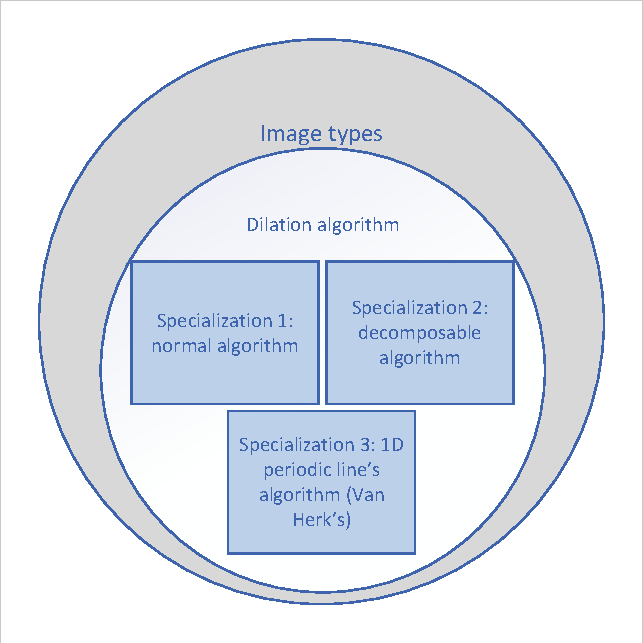
\includegraphics[width=0.99\textwidth]{../figures/dilation_specialization_diagram}
  \end{columns}
\end{frame}

\begin{frame}[fragile]{Taxonomy for Image Processing: Three families}
  \begin{itemize}
    \item Pixel-wise algorithms: thresholding, gamma correction.
    \item Local algorithms: dilation, erosion, closing, hit-or-miss, gradient, rank filter, union-find, max-tree, etc.
    \item Global algorithms: Chamfer distance transform, labeling, etc.
  \end{itemize}
\end{frame}

\begin{frame}[fragile]{Taxonomy for Image Processing: Algorithms canvas}
  \begin{itemize}
    \item Algorithms can have the same shape
    \item When this shape is known, a canvas can be written
    \item This canvas will only require to be provided callbacks for each customization point to work
    \item This canvas can leverage a multitude of implementations techniques to improve performances
  \end{itemize}
\end{frame}

\begin{frame}[fragile]{Taxonomy for Image Processing: Dilation \& Erosion}
  Dilation and Erosion have the same shape:
  \begin{columns}[T,onlytextwidth]
    \column{0.50\textwidth}
    \includegraphics[width=0.7\textwidth]{../figures/dilation_code}

    \column{0.50\textwidth}
    \includegraphics[width=0.7\textwidth]{../figures/erosion_code}
  \end{columns}
  \bigskip
  They can be rewritten in a common canvas:
  \begin{columns}[T,onlytextwidth]
    \column{0.50\textwidth}
    \includegraphics[width=1.1\textwidth]{../figures/local_op_code}

    \column{0.50\textwidth}
    \includegraphics[width=0.6\textwidth]{../figures/local_op_dilation_code}
    \includegraphics[width=0.6\textwidth]{../figures/local_op_erosion_code}
  \end{columns}
\end{frame}

\begin{frame}[fragile]{Taxonomy for Image Processing: Generic canvas}
  Here is how we can write a generic canvas for local algorithms:
  \begin{columns}[T,onlytextwidth]
    \column{0.50\textwidth}
    \begin{minted}{python}
def local_canvas(img, out, se):
  # do something before outer loop
  for pnt in img.points():
    # do something before inner loop
    for nx in se(pnt):
      # do something inner loop
    # do something after inner loop
  # do something after outer loop
\end{minted}

    \column{0.50\textwidth}
    \begin{minted}{python}
def dilate(img, out, se):
  do_nothing = lambda *args, **kwargs: None

  def before_inner_loop(img, out, pnt):
    out(pnt) = img(pnt)

  def inner_loop(ipix, opix, nx):
    out(pnt) = max(out(pnt), img(nx))

  local_canvas(img, out, se,
    before_outer_loop = do_nothing,
    before_inner_loop = before_inner_loop,
    inner_loop        = inner_loop,
    after_inner_loop  = do_nothing,
    after_outer_loop  = do_nothing
  )
\end{minted}
  \end{columns}
\end{frame}

\subsection[Our Concepts for Image Processing]{Our Concepts for Image Processing}

\begin{frame}[fragile]{Our Concepts for Image Processing: outline}
  \begin{itemize}
    \item Fundamental concepts.
    \item Advanced concepts to manipulate images.
    \item Concept support for local algorithms.
  \end{itemize}
\end{frame}

\begin{frame}[fragile]{Our Concepts for Image Processing: fundamentals}
  Fundamental concepts are necessary to be able to do basic manipulations over an image.
  \begin{itemize}
    \item Value: represent an underlying value type and must support a set of operations.
    \item Point: represent a site in an image to locate a value.
    \item Pixel: represent a pair (Value, Point).
    \item Domain: represent the set of points valid for a given image (definition domain).
    \item Image: represent the algebraic relation \(y = f(x)\) where \(y\) is a value generated by the image \(f\) for
          the input (point) \(x\).
    \item Aside from generating a value, an image can also store a value, as in \(f(x) = y\).
  \end{itemize}
\end{frame}

\begin{frame}[fragile]{Our Concepts for Image Processing: fundamentals}
  The basic use case of an image is illustrated by the following code:
  \begin{minted}{C++}
    auto ima = Image();           // Get an image
    for(auto pix : ima.pixels()) {  // Traverse the image
      auto pnt = pix.point();       // Get the pixel's point
      auto& val = pix.value();      // Get the pixel's value
      val = 42;                     // Set the pixel's value
    }
  \end{minted}
\end{frame}

\begin{frame}[fragile]{Our Concepts for Image Processing: Image concept}
  \centering
  \begin{figure}
    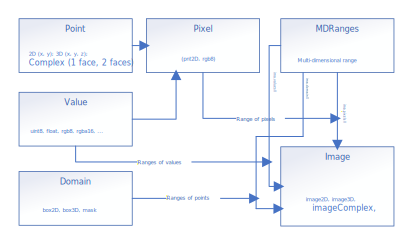
\includegraphics[width=0.9\textwidth]{../figures/concepts/image}
  \end{figure}
\end{frame}

\begin{frame}[fragile]{Our Concepts for Image Processing: Pixel concept}
  \centering
  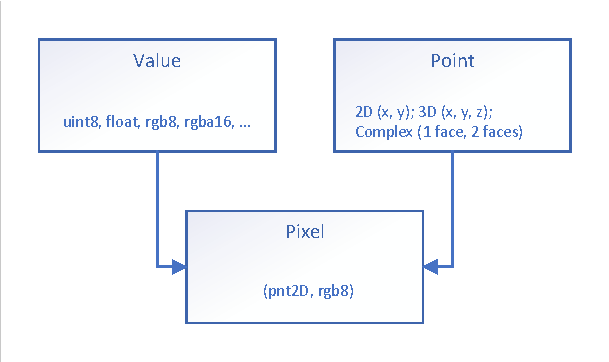
\includegraphics[width=0.5\textwidth]{../figures/concepts/pixel}
  \begin{minted}{C++}
  auto pix = Pixel();     // Get a pixel
  auto val = pix.val();   // yield the pixel value
  auto pnt = pix.point(); // yield the pixel point
  pix.val() = 42;         // Assign a value
  \end{minted}
\end{frame}

\begin{frame}[fragile]{Our Concepts for Image Processing: Domain concept}
  \centering
  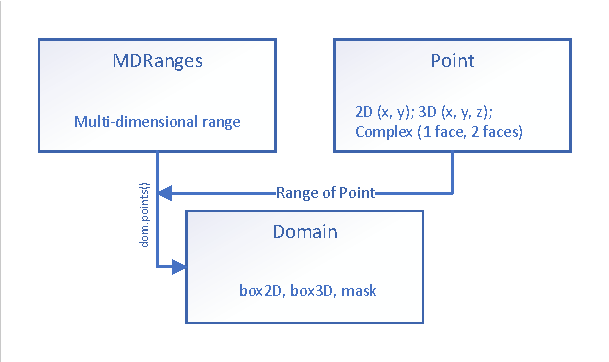
\includegraphics[width=0.45\textwidth]{../figures/concepts/domain}
  \begin{minted}{C++}
    auto dom = Domain();          // Get a domain
    auto pnt = Point(..., ...);   // Get a random point
    bool ret = dom.has(pnt);      // Check wether the domain contains the point
    bool is_empty = dom.empty();  // Check wether the domain is empty
    auto dim = dom.dim();         // Yield the domain's dimension information
    for(auto pnt : dom)           // browse the definition domain
      // use pnt as a point of the domain
  \end{minted}
\end{frame}

\begin{frame}[fragile]{Efficient way to traverse an image}
  Introducing segmented ranges (cf. issues std::mdspan)
  \begin{columns}[T,onlytextwidth]
    \column{0.50\textwidth}
    \begin{figure}
      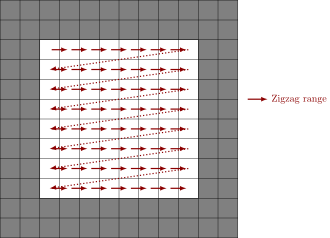
\includegraphics[width=0.8\textwidth]{../figures/linear_rng}
      \caption{Range-v3's ranges}
    \end{figure}

    \column{0.50\textwidth}
    \begin{figure}
      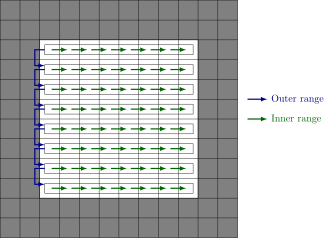
\includegraphics[width=0.8\textwidth]{../figures/segmented_rng}
      \caption{Segmented ranges}
    \end{figure}
  \end{columns}
\end{frame}

\begin{frame}[fragile]{Efficient way to traverse an image}
  Compiler needs explicit contiguous dimension in code to generate vectorized instructions.
  \begin{columns}[T,onlytextwidth]
    \column{0.50\textwidth}
    Unvectorized algorithm:
    \begin{minted}{C++}
template<class I, , class SE>
auto dilate(I input, const SE& se) {
  auto output = input.concretize(); // clone image
  for(auto [in_px, out_px] :
        view::zip(f.pixels(), g.pixels()))
  {
    out_px.val() = out_px.val();
    for(auto nhx : se(in_px))
      out_pix.val() =
        std::max(nhx.val(), out_px.val());
  }
  return output;
}
    \end{minted}
    \column{0.50\textwidth}
    Vectorized algorithm:
    \begin{minted}[highlightlines={7-10}]{C++}
template<class I, class SE>
auto dilate(I input, const SE& se) {
  auto output = input.concretize(); // clone image
  // this line is needed to avoid dangling reference
  auto zipped_pixels =
        view::zip(input.pixels(), output.pixels());
  // unroll the contiguous segments
  for(auto&& row : ranges::rows(zipped_pixels))
    // optimized traversing of the segment
    for(auto [in_px, out_px] : row) {
      out_px.val() = out_px.val();
      for(auto nhx : se(in_px))
        out_pix.val() =
          std::max(in_px.val(), out_px.val());
    }
  return output;
}
    \end{minted}
  \end{columns}
\end{frame}

\begin{frame}[fragile]{Our Concepts for Image Processing: Advanced Image concept}
  \begin{itemize}
    \item IndexableImage: traversing an image via indexes.
    \item AccessibleImage: accessing image's value through points.
    \item BidirectionalImage: traversing image forward and backward.
    \item RawImage: direct access to the image's data buffer.
  \end{itemize}
\end{frame}

\begin{frame}[fragile]{Our Concepts for Image Processing: Advanced Image concept}
  \centering
  \begin{figure}
    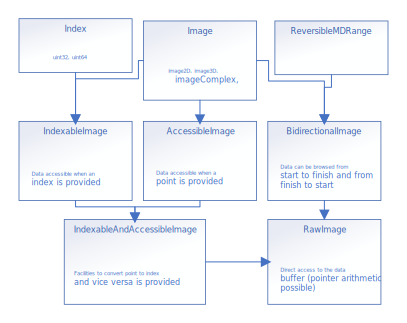
\includegraphics[width=0.7\textwidth]{../figures/concepts/images_all}
  \end{figure}
\end{frame}


\begin{frame}[fragile]{Our Concepts for Image Processing: Local algorithms}
  \begin{itemize}
    \item Support for structuring elements (disc, rectangle, sphere, cube, etc.)
    \item Support for extension (flat buffer, unique value, mirroring, etc.)
  \end{itemize}
  Typical usage in local algorithms:

  \begin{minted}{C++}
      auto se = se::disc(.radius=3); // get a structuring element
      for(auto pix : ima.pixels())   // traverse image
        for(auto nb : se(pix))       // traverse neighboring pixels
          // ...
  \end{minted}
\end{frame}

\begin{frame}[fragile]{Our Concepts for Image Processing: Local algorithms}
  \centering
  \begin{figure}
    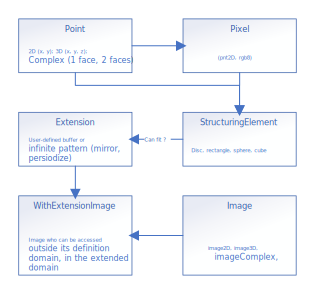
\includegraphics[width=0.7\textwidth]{../figures/concepts/se_extension}
  \end{figure}
\end{frame}

%
%
%
\section[Views for Image Processing]{Views for Image Processing}

\subsection{Genesis of a new abstraction layer: Views}

\begin{frame}[fragile]{Views for Image Processing: outline}
  \begin{itemize}
    \item Genesis of a new abstraction layer: Views
    \item Views for Image Processing
    \item View properties
    \item Use-case: border-management
    \item Limitations \& performance discussion
  \end{itemize}
\end{frame}

\begin{frame}[fragile]{Views for Image Processing: Genesis}
  Inspired from Milena morphers~\footcite{levillain.2009.ismm} and STL ranges~\footcite{niebler.2014.ranges}.
  We published our take in~\footcite[]{roynard.2022.gpce}.
  \begin{alertblock}{View properties}
    \begin{itemize}
      \item Cheap-to-copy
      \item Non-owning (of the data buffer)
      \item Lazy evaluation
      \item Composability
    \end{itemize}
  \end{alertblock}
\end{frame}

\begin{frame}[fragile]{Views for Image Processing: Raising abstraction level}
  Views enable the Image Processing practitioner to rewrite the following alpha-blending algorithm at image level.
  \begin{minted}{C++}
  void blend_inplace(const uint8_t* ima1, uint8_t* ima2, float alpha,
  int width, int height, int stride1, int stride2) {
    for (int y = 0; y < height; ++y) {
      const uint8_t* iptr = ima1 + y * stride1;
      uint8_t* optr = ima2 + y * stride2;
      for (int x = 0; x < width; ++x)
        optr[x] = iptr[x] * alpha + optr[x] * (1-alpha);
    }
  }
  \end{minted}
  \centering
  \begin{figure}
    \includegraphics[width=0.7\textwidth]{../figures/alphablend}
  \end{figure}
\end{frame}

\begin{frame}[fragile]{Views for Image Processing: Raising abstraction level}
  Views can be represented as an expression tree:

  \begin{columns}[T,onlytextwidth]
    \column{0.45\textwidth}
    \centering
    \begin{figure}
      \includegraphics[width=0.7\textwidth]{../figures/view_ast2}
    \end{figure}

    \column{0.55\textwidth}
    \begin{minted}{C++}
auto alphablend =
[](auto ima1, auto ima2, float alpha) {
  return alpha * ima1 +
                (1 - alpha) * ima2;
};
  \end{minted}
  \end{columns}

  \begin{alertblock}{Usage:}
    \begin{minted}{C++}
auto ima1, ima2 = /* ... */;
auto ima_blended = alphablend(ima1, ima2, 0.2);
    \end{minted}
  \end{alertblock}

  \begin{alertblock}{Composability:}
    \begin{minted}{C++}
auto roi = /* ... */;
auto blend_roi = alphablend(view::clip(ima1, roi), view::clip(ima2, roi), 0.2);
auto blend_red = alphablend(view::red(ima1), view::red(ima2), 0.2);
    \end{minted}
  \end{alertblock}

\end{frame}

\begin{frame}[fragile]{Views for Image Processing: Overview}
  \begin{alertblock}{Domain-restrictive views:}
    Filter, clip and mask
    \begin{minted}{C++}
mln::image2d<mln::rgb8> ima = /* ... */ ;
auto mask1 = ima > 125;
auto mask2 = ima <= 125;
mln::fill(mln::view::mask(ima, mask1), 255); // Thresholding
mln::fill(mln::view::mask(ima, mask2), 0);
    \end{minted}
  \end{alertblock}

  \begin{alertblock}{Value-transforming view:}
    Transform, zip, channel projectors, conversion (cast), operators (arithmetical, logical, mathematical)
    \begin{minted}{C++}
mln::image2d<uint8_t> ima = /* ... */ ;
auto ero = erode(ima);
auto dil = dilate(ima);
uint8_t zero = 0;
auto ret = mln::view::ifelse(dil < ero, ero - dil, zero); // Hit-or-miss
    \end{minted}
  \end{alertblock}
\end{frame}

\begin{frame}[fragile]{Views for Image Processing: Properties}
  \centering
  \begin{figure}
    \includegraphics[width=0.9\textwidth]{../figures/view_property}
  \end{figure}
\end{frame}

\begin{frame}[fragile]{Views for Image Processing: Concrete Use-case --- background subtraction}
  \begin{figure}[htbp]
    \centering
    \includegraphics[width=0.9\linewidth]{../figures/pipeline_bg_sub_comp}
    \caption{Background subtraction pipeline using \colorbox{lightgreen}{algorithms} and
      \colorbox{thistle}{views}.}
  \end{figure}
\end{frame}

\begin{frame}[fragile]{Views for Image Processing: Concrete Use-case --- background subtraction}
  \begin{figure}[htbp]
    \centering
    \begin{tabular}{cccc}
      Background                                                                        & Candidate & Result                     \\[5pt]
      \fbox{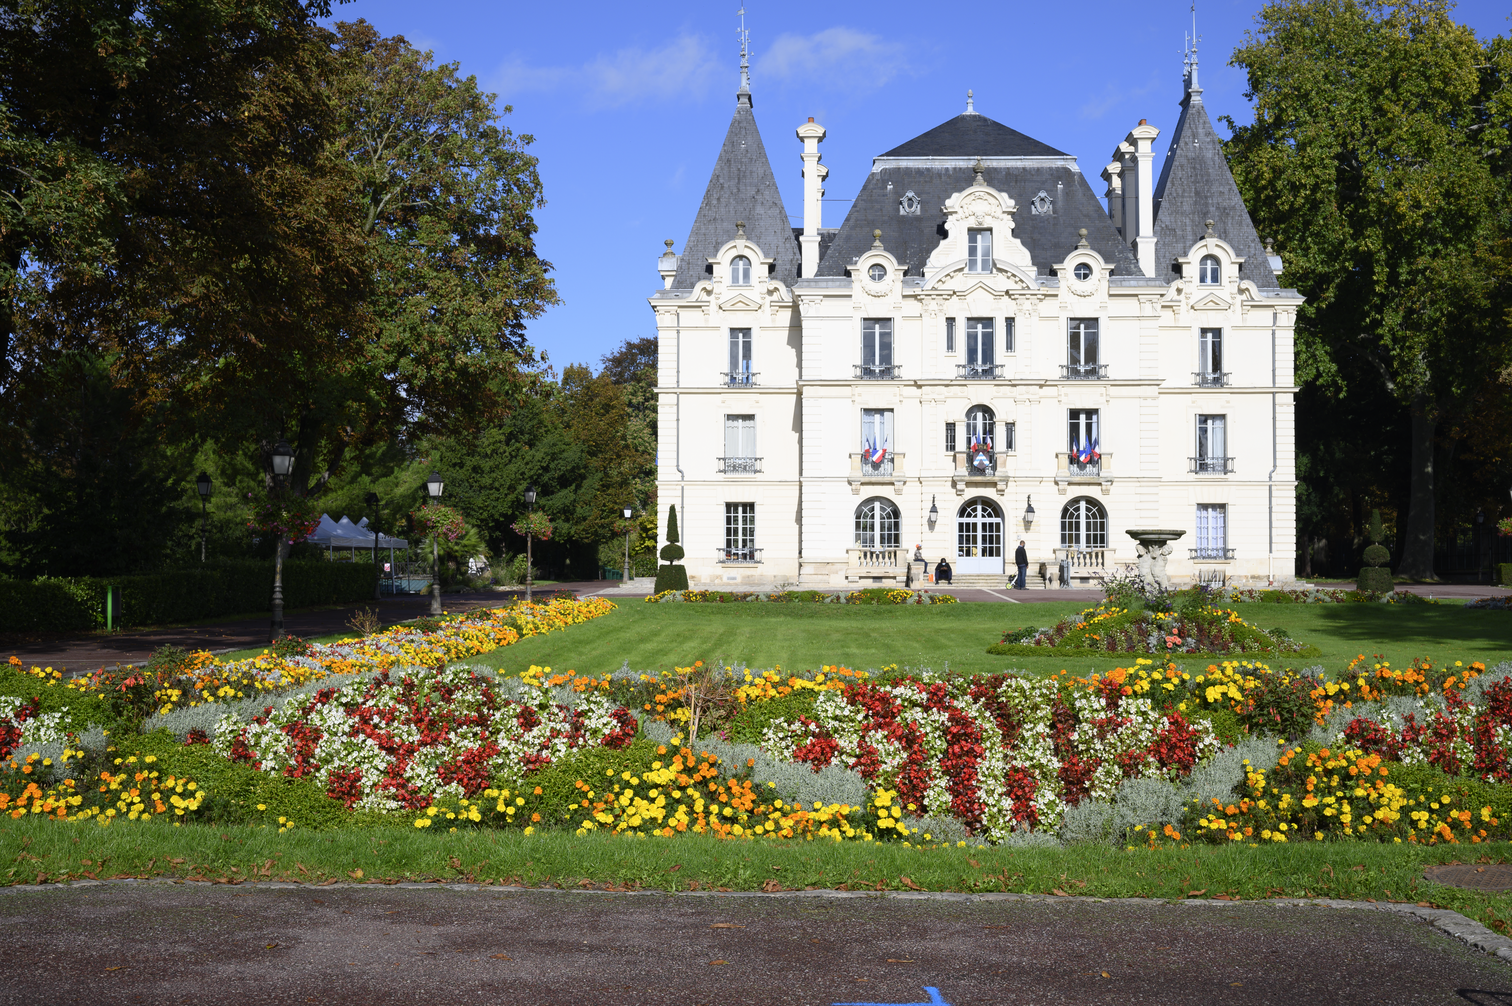
\includegraphics[width=.25\linewidth]{../assets/1512x1006/castle_bg.png}}   &
      \fbox{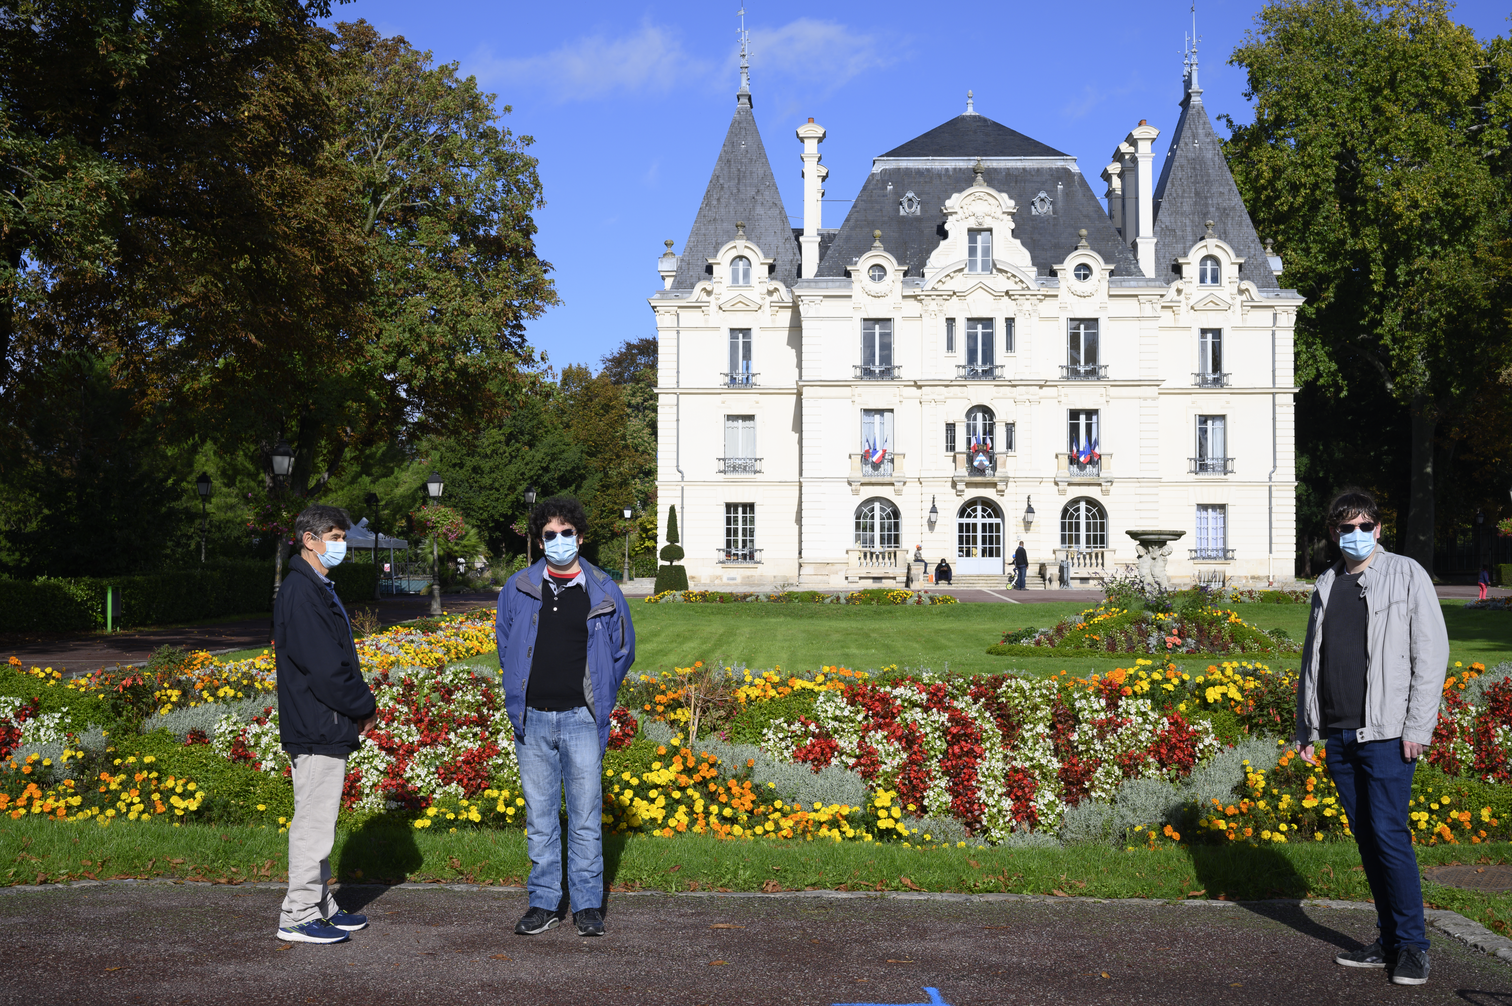
\includegraphics[width=.25\linewidth]{../assets/1512x1006/castle_fg_1.png}} &
      \fbox{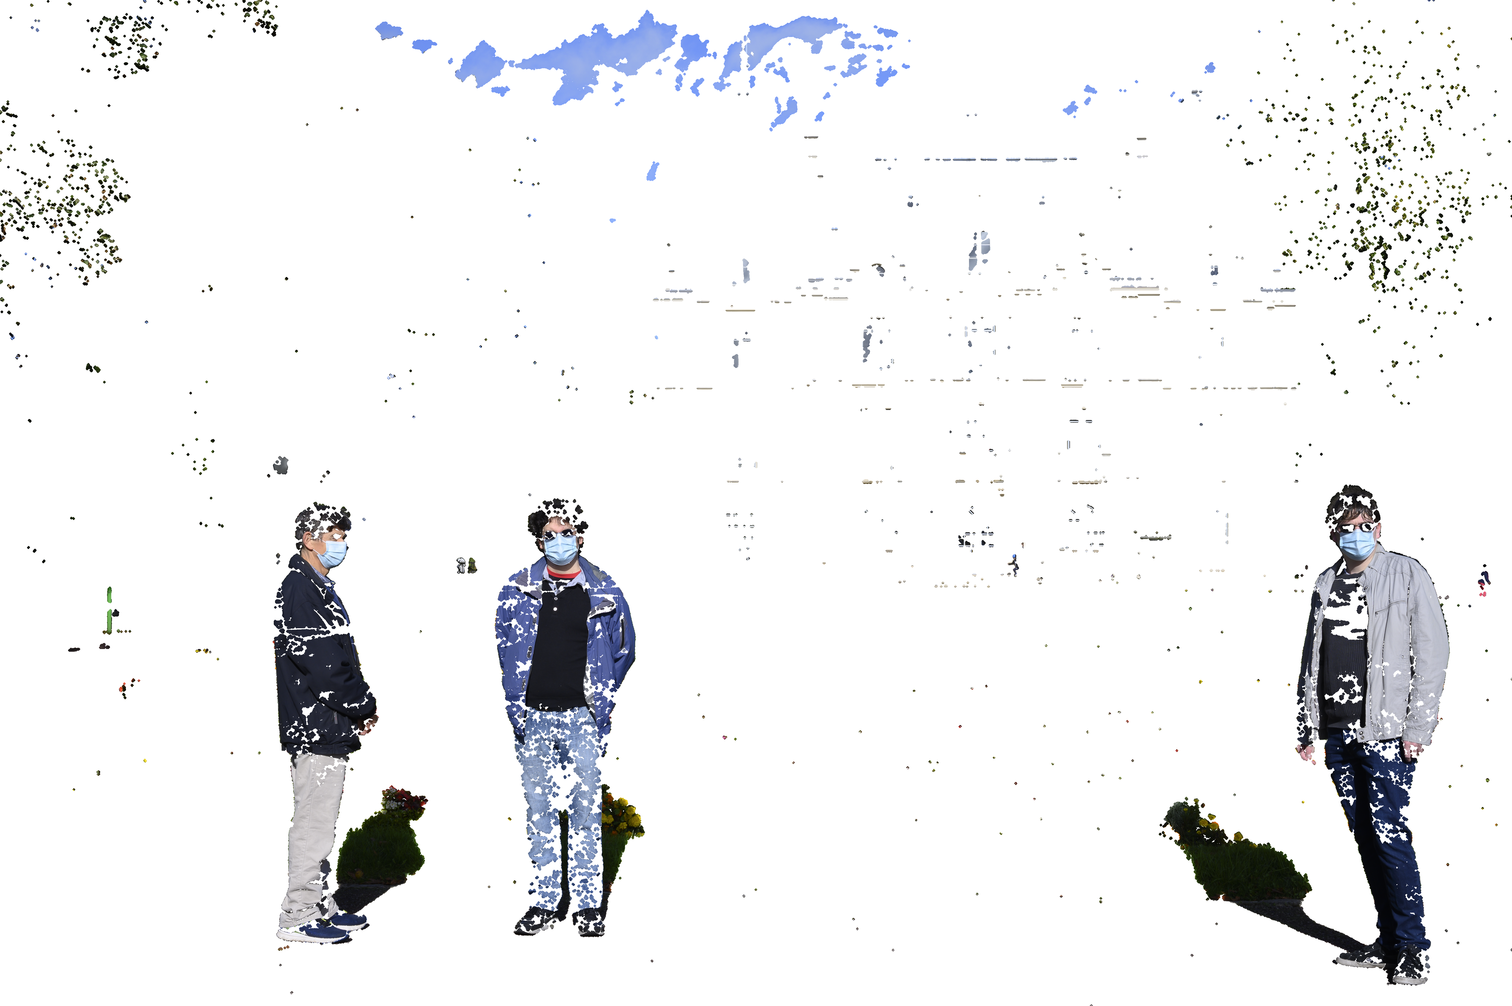
\includegraphics[width=.25\linewidth]{../assets/1512x1006/results_sig1_win5/castle/result_detected_castle_fg_1.png}} \\[5pt]
      \fbox{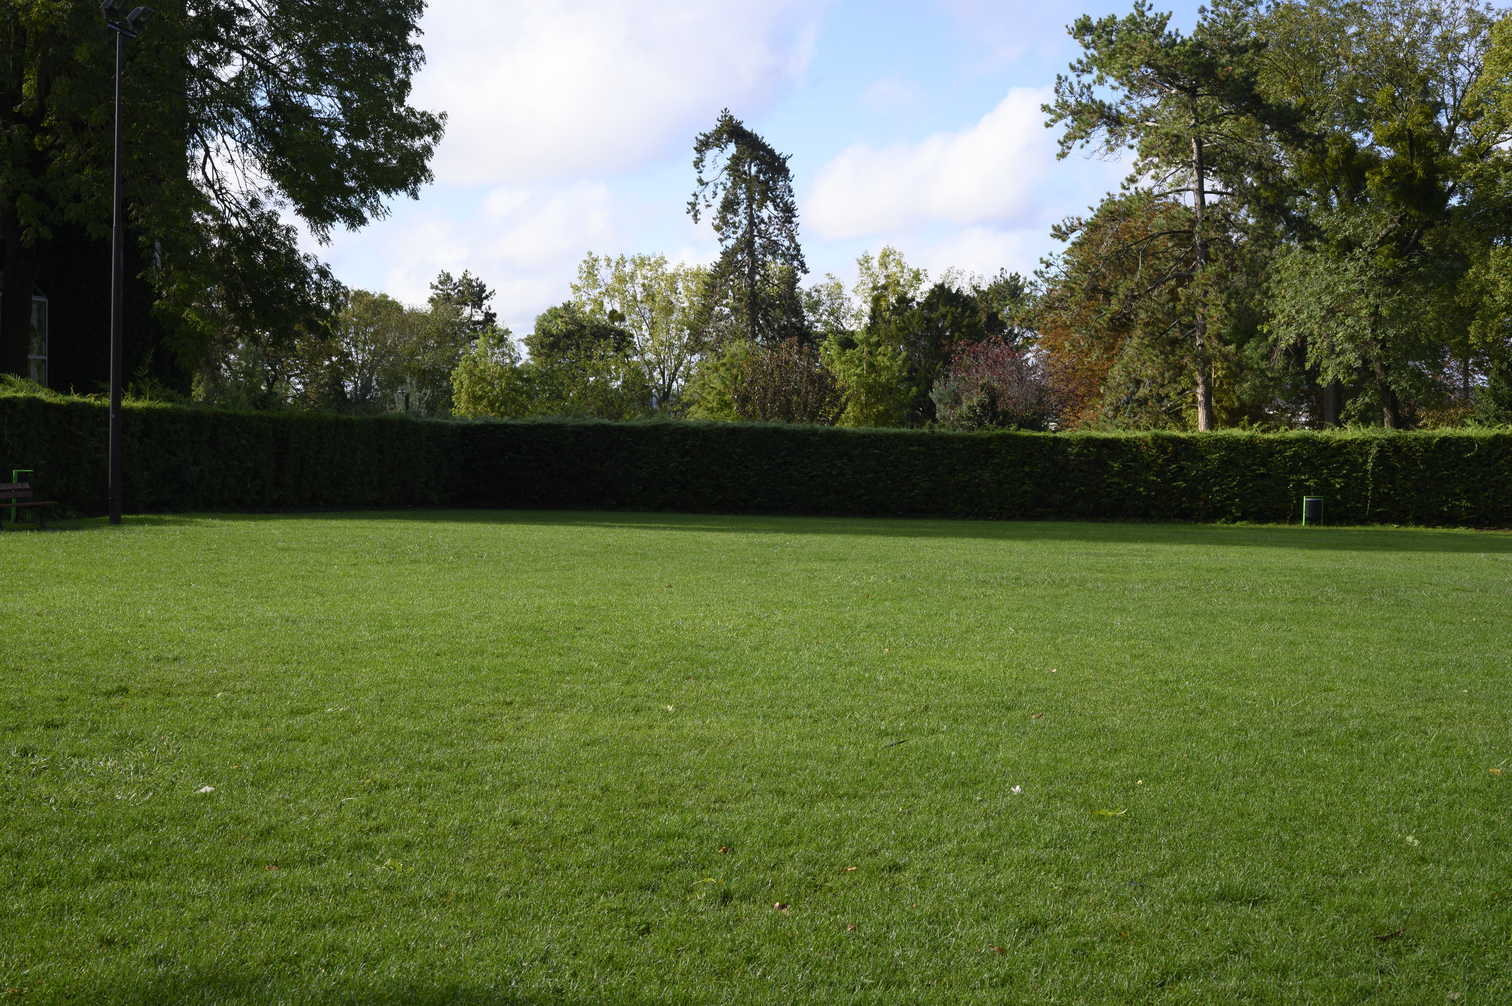
\includegraphics[width=.25\linewidth]{../assets/1512x1006/garden_bg.png}}   &
      \fbox{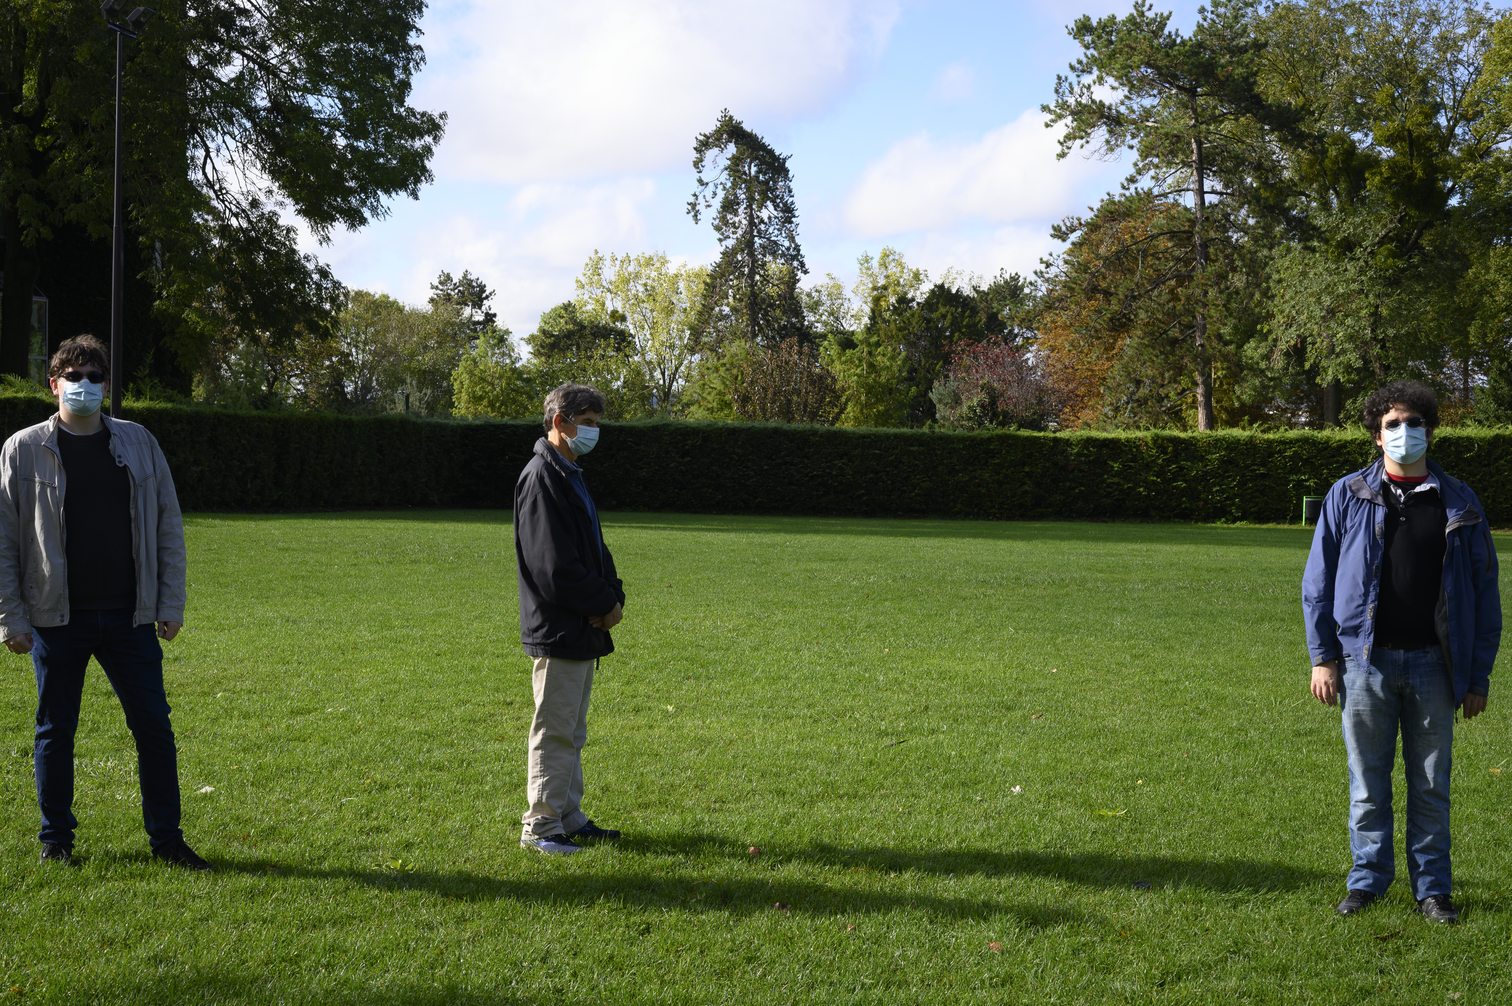
\includegraphics[width=.25\linewidth]{../assets/1512x1006/garden_fg_1.png}} &
      \fbox{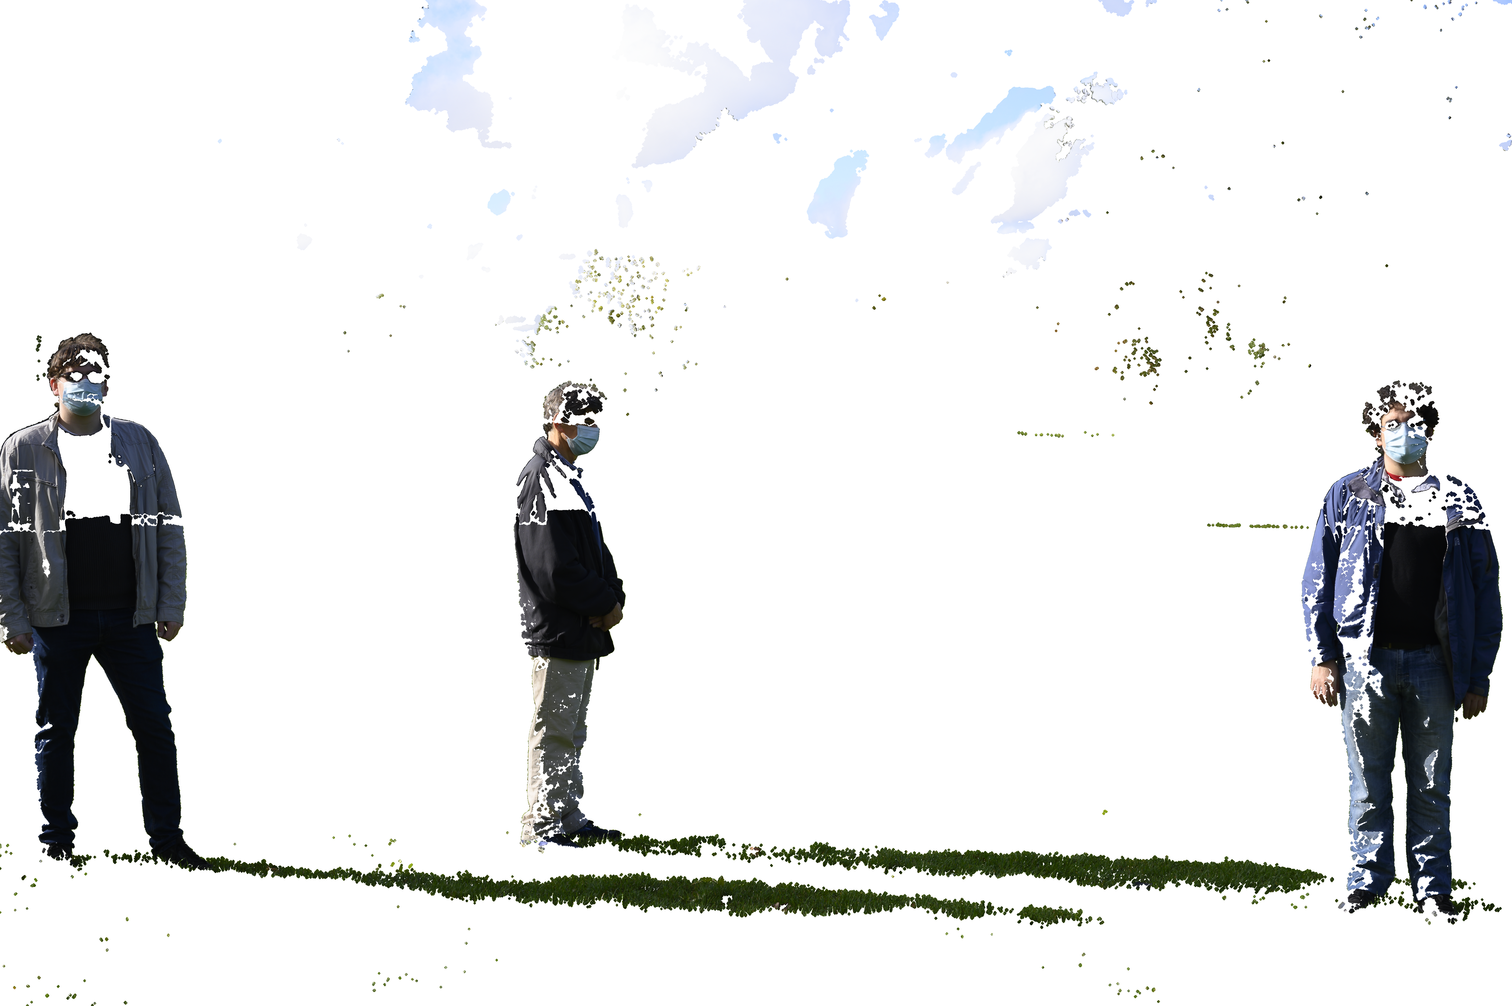
\includegraphics[width=.25\linewidth]{../assets/1512x1006/results_sig1_win5/garden/result_detected_garden_fg_1.png}}
    \end{tabular}

    \caption{Background detection: data set samples.}
    \label{fig:bg_sub.dataset_samples}
  \end{figure}
\end{frame}

\newcommand{\mystd}[1]{{\itshape(\(\pm\) #1)}}
\newcommand{\mydelta}[1]{{\itshape\bfseries #1\%}}

\begin{frame}[fragile]{Views for Image Processing: Concrete Use-case --- background subtraction}
  \begin{figure}
    \begin{minted}[highlightlines={3-4,6,8},highlightcolor=thistle]{c++}
    float kThreshold = 150; float kVSigma = 10;
    float kHSigma = 10;  int kOpeningRadius = 32;
    auto img_gray = view::transform(img_color, to_gray);
    auto bg_gray  = view::transform(bg_color, to_gray);
    auto bg_blurred = gaussian2d(bg_gray,  kHSigma, kVSigma);
    auto tmp_gray = img_gray - bg_blurred;
    auto thresholdf = [](auto x) { return x < kThreshold; };
    auto tmp_bin = view::transform(tmp_gray, thresholdf);
    auto ero = erosion(tmp_bin, disc(kOpeningRadius));
    dilation(ero, disc(kOpeningRadius), output);
    \end{minted}
    \caption{Pipeline implementation with \colorbox{thistle}{\emph{views}}. Highlighted code uses \emph{views} by
      prefixing operators with the namespace \texttt{view}.}
    \label{fig:view.comp.sub_bg.view_code}
  \end{figure}
\end{frame}

\begin{frame}[fragile]{Views for Image Processing: Concrete Use-case --- background subtraction}
  \begin{table}
    \centering
    \begin{tabular}{l|ccc}
      \toprule
      Framework          & Compute Time            & Memory usage & \(\Delta{}\)Memory usage \\ \midrule
      Pylene (w/o views) & \(2.11s\) \mystd{144ms} & 106 MB       & \mydelta{+0}             \\
      OpenCV             & \(2.41s\) \mystd{134ms} & 59 MB        & \mydelta{-44}            \\
      Pylene (views)     & \(2.13s\) \mystd{164ms} & 51 MB        & \mydelta{-52}            \\
      \bottomrule
    \end{tabular}
    \caption{Benchmarks of the previous pipeline on a dataset (12 images) of 10MPix images. Average
      computation time and memory usage of implementations with/without \emph{views} and with OpenCV as a baseline.}
    \label{table:views.perf}
    %\vspace{-1em}
  \end{table}
\end{frame}

%
%
%
\section{General Conclusion \& Continuation}

\begin{frame}{Static-dynamic bridge}
  TODO
\end{frame}

\begin{frame}{Conclusion}
  TODO
\end{frame}

\begin{frame}[allowframebreaks]{Publications}
  \small
  \begin{itemize}
    \item \fullcite{roynard.2019.rrpr}
    \item \fullcite{roynard.2022.gpce}
  \end{itemize}
\end{frame}

{\setbeamercolor{palette primary}{fg=black, bg=lightgray}
\begin{frame}[standout]
  Questions?
\end{frame}
}

\appendix

\begin{frame}[allowframebreaks]{References}
  \printbibliography[heading=none]
\end{frame}

%\begin{frame}[fragile]{Backup slides}
%  Sometimes, it is useful to add slides at the end of your presentation to
%  refer to during audience questions.
%
%  The best way to do this is to include the \verb|appendixnumberbeamer|
%  package in your preamble and call \verb|\appendix| before your backup slides.
%
%  \themename will automatically turn off slide numbering and progress bars for
%  slides in the appendix.
%\end{frame}

\end{document}